\documentclass[conference, a4paper]{IEEEtran}

% --- CÁC GÓI THƯ VIỆN CẦN THIẾT ---
\usepackage{cite}
\usepackage{amsmath,amssymb,amsfonts}
\usepackage{microtype}
\usepackage{algorithmic}
\usepackage{graphicx}
\usepackage{textcomp}
\usepackage{xcolor}
\usepackage[utf8]{inputenc}
\usepackage[T1]{fontenc}
\usepackage[bookmarks=false, draft]{hyperref}
\usepackage{url}
\usepackage[top=0.75in, bottom=1in, left=0.625in, right=0.625in]{geometry}
\setlength{\columnsep}{0.24in}
\begin{document}

% --- TIÊU ĐỀ BÀI BÁO ---
\title{Med-TCAX: Tier-Constrained Causal-Argumentative Explainability for Clinical Machine Learning}

% --- THÔNG TIN TÁC GIẢ (Đẩy sang trái theo đúng ảnh mẫu) ---
\author{
\IEEEauthorblockN{Nguyen Nhat Huy}
\IEEEauthorblockA{\textit{Department of Artificial Intelligence} \\
\textit{FPT University}\\
Ha Noi, Vietnam \\
nguyenhuy07032006@gmail.com}
\and
\IEEEauthorblockN{Nguyen Xuan Thang}
\IEEEauthorblockA{\textit{Department of Artificial Intelligence} \\
\textit{FPT University}\\
Ha Noi, Vietnam \\
lumberwack24@gmail.com}
\and
\IEEEauthorblockN{Ngo Nguyen Khanh Huy}
\IEEEauthorblockA{\textit{Department of Artificial Intelligence} \\
\textit{FPT University}\\
Ha Noi, Vietnam \\
huyngonguyenkhanh@gmail.com}
\and
\IEEEauthorblockN{Cao Van Mai}
\IEEEauthorblockA{\textit{Department of Artificial Intelligence} \\
\textit{FPT University}\\
Ha Noi, Vietnam \\
maicv2@fe.edu.vn}
}

\maketitle



% --- TÓM TẮT (ABSTRACT) ---
\begin{abstract}
The integration of machine learning into clinical decision support requires transparent, medically coherent explanations. Traditional methods like SHAP or LIME lack structural awareness, often producing inconsistent results. While causal discovery algorithms like FCI capture structural dependencies, they frequently yield clinically implausible or unstable graphs. We propose Med-TCAX, a Tier-Constrained Causal-Argumentative explainability framework. Med-TCAX enforces domain-specific medical precedence via tiered constraints and leverages a Bipolar Argumentation Framework (BAF) under semi-stable semantics to produce coherent, human-interpretable reasoning chains. Experimental results on UCI Heart Disease and Pima Indians Diabetes datasets demonstrate that Med-TCAX significantly reduces clinically implausible edges, enhances causal graph stability, and provides more clinically coherent explanations compared to standard feature-attribution baselines.
\end{abstract}

% --- TỪ KHÓA (KEYWORDS) ---
\begin{IEEEkeywords}
 Argumentation Theory, Bipolar Argumentation Framework, Causal Discovery, Clinical Decision Support, Constraint-based Learning, Explainable AI, Hierarchical Causal Modeling, Semi-stable Semantics
\end{IEEEkeywords}

% --- NỘI DUNG CHÍNH ---

\section{Introduction}
The growing adoption of machine learning (ML) in clinical decision support has intensified demand for transparent and interpretable model predictions \cite{ref1}. Clinicians require explanations that are not only faithful to model behavior but also consistent with established biological and temporal knowledge—a requirement that existing post-hoc explainability methods fail to satisfy \cite{ref2}.

Feature-attribution methods such as SHAP \cite{ref3} and LIME \cite{ref4} are widely used but explain predictions in terms of isolated feature contributions without capturing inter-feature structural relationships or causal plausibility. They are additionally sensitive to correlated features and provide no guarantees against temporally reversed or biologically impossible attributions \cite{ref5}.

Constraint-based causal discovery, particularly the Fast Causal Inference (FCI) algorithm \cite{ref6}, offers richer structural explanations through directed graphical models. However, when applied to observational clinical data, discovered graphs frequently contain biologically inconsistent edges---such as outcomes causing their own predictors---due to edge-direction inconsistency and insufficient domain constraints \cite{ref7}. Furthermore, raw causal graphs do not directly yield human-interpretable reasoning chains suitable for clinical explanation.

To address these limitations, we propose Med-TCAX, a tier-constrained causal-argumentative explainability framework. Experiments on the UCI Heart Disease and Pima Indians Diabetes datasets demonstrate that Med-TCAX reduces domain-inconsistent connections, improves graph stability, and produces more coherent explanations than SHAP and LIME baselines. Specifically, the main contributions of this paper are:
\begin{itemize}
    \item A medical variable tiering scheme that encodes biological precedence as forbidden-edge constraints for FCI, significantly reducing clinically implausible causal directions.
    \item A dual-encoding strategy combined with K-Fold cross-validation to mitigate causal orientation artifacts and improve graph stability over discretized variables.
    \item The integration of a Bipolar Argumentation Framework (BAF) with semi-stable semantics to translate the constrained causal graph into structured, conflict-consistent explanations.
\end{itemize}

The remainder of this paper is organized as follows. Section II reviews related work in post-hoc explainability, causal discovery, and argumentation frameworks. Section III details the Med-TCAX methodology. Section IV outlines the experimental setup, while Section V presents the evaluation and comparative analysis. Section VI discusses limitations, and Section VII concludes the paper with directions for future work.

\section{Related Work}

\subsection{Post-hoc Explainable AI}
Post-hoc explainability methods are widely used in clinical machine learning to clarify model predictions after training. SHAP \cite{ref3} explains predictions through Shapley-value-based feature contributions, while LIME \cite{ref4} approximates local model behavior using interpretable surrogate models. Although these methods are practical and model-agnostic, they mainly provide scalar feature attributions. As a result, they do not explicitly model inter-feature dependencies and may produce explanations that are difficult to interpret causally, especially in clinical datasets with correlated predictors \cite{ref5}.

\subsection{Causal Discovery for Explainability}
Causal discovery methods infer structural dependency patterns from observational data \cite{ref12}. The FCI algorithm \cite{ref13} extends causal discovery to partial ancestral graphs (PAGs), which can represent latent confounders and partially oriented causal relations, making it more suitable for observational clinical data. Causal Shapley values \cite{ref15} integrate causal graphs with feature attribution to produce causally consistent importance scores. However, constraint-based methods applied to clinical data remain vulnerable to directional artifacts and spurious edges arising from confounding, yielding PAGs that may violate biological and temporal constraints \cite{ref7}.

\subsection{Background Knowledge in Causal Discovery}
Domain knowledge can constrain the causal search space through forbidden-edge rules, required-edge rules, and temporal priors \cite{ref16}. Meek \cite{ref17} formalized background knowledge integration for constraint-based discovery. Temporal ordering constraints have been applied to longitudinal clinical data via PCMCI \cite{ref18} and tier-based priors \cite{ref19} to prevent reverse-temporal edges. Expert-curated knowledge graphs derived from sources such as UMLS have also been used as causal priors \cite{ref20}. However, many existing applications rely on limited forms of background knowledge, such as outcome-sink constraints that prevent outcome variables from having outgoing edges. Such constraints reduce reverse-temporal artifacts but do not systematically enforce causal plausibility across broader clinical variable categories, leaving many implausible inter-predictor relations unaddressed.

\subsection{Argumentation Frameworks for XAI}
Dung's abstract argumentation framework (AF) \cite{ref21} provides a formal basis for reasoning under conflict, with acceptability defined through extensions such as stable, preferred, and grounded semantics. Bipolar argumentation frameworks (BAF) \cite{ref22} augment AFs with explicit support relations, enabling richer reasoning over reinforcing and conflicting evidence. Semi-stable semantics \cite{ref23} maximize the range of accepted arguments among all admissible extensions, ensuring informative and consistent explanations. Argumentation has been applied to ML explainability through rule-based argument construction \cite{ref24} and contrastive explanation generation \cite{ref25}, though existing approaches do not integrate causal discovery with argumentation or enforce clinical plausibility.

\subsection{Medical Causal Constraints and Clinical Plausibility}
Medical coherence in causal models encompasses biological consistency, temporal causality, and medical variable hierarchy compliance \cite{ref7, ref26}. Domain-inconsistent connections—such as outcomes causing preceding measurements—arise in data-driven causal graphs and can mislead clinical interpretation \cite{ref27}. Prior approaches include temporal constraint graphs \cite{ref18}, ontology-based causal priors \cite{ref20}, and counterfactual consistency constraints \cite{ref28}. However, these methods typically focus on predictor-outcome relationships and require exhaustive edge-level annotation that does not scale to high-dimensional clinical datasets. Med-TCAX addresses this gap with a scalable tier-based constraint scheme that enforces plausibility across all variable categories without requiring manual per-edge specification.

\section{Methodology}

\subsection{Overview}

This study proposes a tier-constrained causal-argumentation framework for explainable machine learning. The proposed methodology is evaluated using the \textit{heart\_disease} dataset as a running reference case. The purpose of this dataset is not to establish a deployable clinical diagnosis system, but to demonstrate how causal discovery, semantic constraints, and argumentation-based inference can be integrated into a coherent explainability pipeline. The accompanying implementation is available in the GitHub repository \cite{github_repo}.


As shown in Fig.~\ref{fig:overall_pipeline}, the framework consists of three main processing layers following the overview stage:

\begin{enumerate}
    \item K-Fold Stability Discovery Layer,
    \item Semantics Filter Layer,
    \item Argumentative Inference Layer.
\end{enumerate}

The first layer discovers causal relations that remain stable across K-Fold splits and alternative encoding strategies. The second layer applies medical tier constraints to remove semantically implausible directions. The third layer transforms the final causal graph into an argumentation framework and computes argument acceptance under semi-stable semantics.

\begin{figure*}[htbp]
    \centering
    
\includegraphics[width=\textwidth]{figures/pipeline.png}
    \caption{Overall architecture of the proposed tier-constrained causal-argumentation framework.}
    \label{fig:overall_pipeline}
\end{figure*}

\subsubsection{Reference Dataset and Scalability Screening}

The \textit{heart\_disease} dataset is used as a reference dataset to trace all stages of the framework. The target variable is denoted as $Y$, while the input variables are denoted as:

\begin{equation}
X = \{X_1, X_2, \ldots, X_p\}.
\end{equation}

For datasets with a large number of variables, an initial SHAP-based feature screening step is used before causal discovery. This step is introduced only as a computational scalability mechanism. It reduces the candidate feature set to the most influential variables before FCI-based discovery is performed. In this study, a maximum of 11 features is retained for large datasets because causal discovery and argumentation construction become computationally expensive when the number of variables exceeds this range.

The SHAP screening result for the \textit{heart\_disease} reference case is shown in Fig.~\ref{fig:heart_shap}. Importantly, SHAP is not treated as the final explanation method in this framework. Instead, it is used as a preliminary feature filtering mechanism. The final explanation is produced by the causal-argumentation pipeline.

\begin{figure}[htbp]
    \centering
    
\includegraphics[width=\linewidth]{figures/heart_disease_shap_bar.png}
    \caption{SHAP-based feature screening for the \textit{heart\_disease} reference dataset. For large datasets, this step is used to retain a computationally manageable candidate feature set before causal discovery.}
    \label{fig:heart_shap}
\end{figure}

% ======================================================

\subsection{K-Fold Stability Discovery Layer}

The goal of this layer is to identify causal relations that are robust to data splitting and dummy-variable encoding choices. This is necessary because causal discovery over encoded categorical variables may produce unstable edges when different dummy columns are selected as reference categories.

\subsubsection{K-Fold Data Splitting}

Given a dataset $D$, the data is partitioned into $K$ folds:

\begin{equation}
D = \{D_1, D_2, \ldots, D_K\}.
\end{equation}

For each fold $k$, the training subset is used to perform causal discovery. This process reduces the risk that the final graph is dominated by fold-specific sampling artifacts.

\subsubsection{Dual Encoding Strategy}

For each fold, two encoded versions of the same data are generated:

\begin{equation}
D_k^{drop\text{-}first}, \qquad D_k^{drop\text{-}last}.
\end{equation}

The drop-first and drop-last strategies produce different dummy-variable representations for categorical variables. Running causal discovery under both encodings helps reduce encoding-dependent artifacts. If a relation only appears under one arbitrary encoding choice, it is considered less reliable than a relation that remains stable across encoding variants.

\subsubsection{Fold-Level FCI Discovery}

The Fast Causal Inference algorithm is applied separately to each encoded dataset:

\begin{equation}
G_k^{first} = FCI(D_k^{drop\text{-}first}),
\end{equation}

\begin{equation}
G_k^{last} = FCI(D_k^{drop\text{-}last}).
\end{equation}

FCI is used because it can represent uncertainty in causal direction and allows for the possibility of latent confounders. The output of this step is a fold-specific causal structure over encoded variables.

\subsubsection{Group-Level Edge Extraction}

Because dummy variables are only encoded representations of original variables, edges between encoded variables are mapped back to their original feature groups. Let $g(v)$ denote the original feature group of an encoded variable $v$. An encoded edge $(u,v)$ is converted into a group-level relation:

\begin{equation}
(g(u), g(v)).
\end{equation}

The fold-level group edge set is therefore defined as:

\begin{equation}
E_k = \{(X_i, X_j) \mid X_i \neq X_j\}.
\end{equation}

This step prevents the final explanation from being expressed in terms of dummy columns only. Instead, the graph is interpreted at the level of clinically meaningful variables such as \textit{age}, \textit{thalach}, \textit{oldpeak}, \textit{cp}, and \textit{num}.

\subsubsection{Fold-Level Merge}

For each fold, the group-level edges obtained from the two encoding strategies are merged:

\begin{equation}
E_k^{merge} = E_k^{first} \cup E_k^{last}.
\end{equation}

When multiple encoded-variable pairs support the same group-level relation, the strongest associated correlation is retained as the representative relation strength. This produces a more compact fold-level causal structure while preserving the strongest observed association between the corresponding feature groups.

\subsubsection{K-Fold Majority Merge}

After all folds are processed, the merged fold-level edge sets are aggregated using majority voting:

\begin{equation}
E_{\text{stable}} =
\{e \mid \text{freq}(e) \geq \tau\},
\end{equation}

where $\text{freq}(e)$ is the number of folds in which edge $e$ appears, and $\tau$ is the minimum stability threshold. The resulting graph is called the \textbf{Stable Group-Level Causal Graph}.

For the \textit{heart\_disease} reference case, the stable group-level directions are visualized in Fig.~\ref{fig:merged_group_directions}. For example, the graph retains clinically interpretable relations such as \textit{age} $\rightarrow$ \textit{trestbps}, \textit{age} $\rightarrow$ \textit{thalach}, \textit{cp} $\rightarrow$ \textit{num}, \textit{oldpeak} $\rightarrow$ \textit{num}, and \textit{thal} $\rightarrow$ \textit{num}. Edge labels indicate the strongest representative correlation selected from the corresponding encoded-variable pairs.

\begin{figure}[htbp]
    \centering
    
\includegraphics[width=\linewidth]{figures/merged_group_directions.png}
    \caption{Stable group-level causal directions obtained from K-Fold majority merging on the \textit{heart\_disease} reference dataset. Edge labels show the strongest representative correlation between encoded-variable pairs.}
    \label{fig:merged_group_directions}
\end{figure}

% ======================================================

\subsection{Semantics Filter Layer}

The purpose of this layer is to ensure that the discovered causal directions remain semantically plausible under medical domain knowledge. While K-Fold stability improves statistical robustness, it does not by itself guarantee that every direction is clinically meaningful. Therefore, tier-based constraints are introduced as background knowledge.

\subsubsection{Tier Definition}

Variables are assigned into ordered semantic tiers. In the \textit{heart\_disease} reference case, the variables can be grouped as follows:

\begin{itemize}
    \item Tier 1: demographic or baseline variables, e.g., \textit{age}, \textit{sex};
    \item Tier 2: clinical examination and test variables, e.g., \textit{trestbps}, \textit{thalach}, \textit{oldpeak}, \textit{cp}, \textit{exang}, \textit{ca}, \textit{thal};
    \item Tier 3: clinical outcome variable, e.g., \textit{num}.
\end{itemize}

The tier ordering encodes the assumption that earlier-tier variables may influence later-tier variables, while later-tier variables should not causally determine earlier-tier variables.

\subsubsection{Background Knowledge Construction}

The tier definitions are converted into background knowledge constraints for causal discovery. A directed relation from $X_j$ to $X_i$ is forbidden whenever $X_j$ belongs to a later tier than $X_i$:

\begin{equation}
X_j \rightarrow X_i \quad \text{is forbidden if} \quad
T(X_j) > T(X_i),
\end{equation}

where $T(X)$ denotes the tier index of variable $X$.

This constraint prevents implausible directions such as the disease outcome causing demographic attributes. As a result, the Semantics Filter Layer acts as a domain-level correction mechanism on top of the stability-based graph discovery process.

\subsubsection{Full-Data Unified Encoding}

After stable group-level relations have been identified, the full dataset is encoded using a unified encoding scheme. This produces a consistent encoded representation:

\begin{equation}
D^{U} = Encode(D).
\end{equation}

The purpose of this step is not to rediscover all causal relations from scratch. Instead, the unified encoded dataset provides a common representation onto which the stable group-level relations can be projected.

\subsubsection{Final Unified Encoded Graph}

The final graph is constructed by projecting the stable group-level causal relations onto the unified encoded variables:

\begin{equation}
G_{\text{final}} = (V^{U}, E_{\text{final}}),
\end{equation}

where $V^{U}$ is the set of unified encoded variables and $E_{\text{final}}$ is derived from $E_{\text{stable}}$ after semantic filtering and encoded-level projection.

For the \textit{heart\_disease} reference case, the final unified encoded graph is shown in Fig.~\ref{fig:final_unified_graph}. This graph contains encoded interval-level arguments such as \textit{trestbps[-inf,143.000)}, \textit{thalach[147.500,inf)}, and \textit{oldpeak[1.700,inf)}. These encoded arguments are later used as the input arguments for the argumentation layer.

\begin{figure}[htbp]
    \centering
    
\includegraphics[width=\linewidth]{figures/final_unified_encoded_graph.png}
    \caption{Final unified encoded graph for the \textit{heart\_disease} reference dataset. Stable group-level causal relations are projected onto the unified encoded representation before argumentation construction. For readability, this figure shows only a cropped portion of the full graph; the complete visualization is available in the accompanying GitHub repository.
}
    \label{fig:final_unified_graph}
\end{figure}

% ======================================================

\subsection{Argumentative Inference Layer}

The Argumentative Inference Layer transforms the final encoded causal graph into an argumentation-based explanation model. This layer is responsible for converting causal relations into support and attack structures and then computing which arguments are accepted under semi-stable semantics.

\subsubsection{Bipolar Argumentation Framework Construction}

The final causal graph is first converted into a Bipolar Argumentation Framework:

\begin{equation}
BAF = (A, R_{sup}, R_{att}),
\end{equation}

where $A$ is the set of arguments, $R_{sup}$ is the set of support relations, and $R_{att}$ is the set of attack relations.

Each encoded variable state is treated as an argument. Positive causal influence is represented as a support relation, while negative causal influence, contradiction, or mutual exclusivity is represented as an attack relation. For example, two encoded intervals from the same original variable are mutually exclusive and therefore cannot be accepted together.

\subsubsection{Conversion to Classical Argumentation Framework}

Because semi-stable semantics are defined over classical Argumentation Frameworks, the BAF is converted into a classical AF:

\begin{equation}
AF = (A, R'_{att}),
\end{equation}

where $R'_{att}$ is the final attack relation after incorporating direct attacks, mutual exclusivity attacks, and attacks induced through support closure.

The unfiltered classical AF is shown in Fig.~\ref{fig:classical_af}. This graph preserves the full interaction structure, but it may contain visually dense relations. Therefore, a filtered version is also produced in Fig.~\ref{fig:classical_af_filtered} to improve interpretability by retaining the most relevant attack relations.

\begin{figure}[htbp]
    \centering
    
\includegraphics[width=\linewidth]{figures/classical_af.png}
    \caption{Classical argumentation framework generated from the final unified encoded causal graph. Nodes represent encoded arguments and edges represent attack relations.}
    \label{fig:classical_af}
\end{figure}

\begin{figure}[htbp]
    \centering
    
\includegraphics[width=\linewidth]{figures/classical_af_filtered.png}
    \caption{Filtered classical argumentation framework. The filtered graph improves readability by emphasizing the most relevant argumentative interactions.}
    \label{fig:classical_af_filtered}
\end{figure}

\subsubsection{Semi-Stable Extension Computation}

Semi-stable semantics are then applied to compute acceptable sets of arguments. Given an argumentation framework $AF$, the set of semi-stable extensions is denoted as:

\begin{equation}
\mathcal{E}_{ss}(AF).
\end{equation}

Each extension $E \in \mathcal{E}_{ss}(AF)$ represents a conflict-consistent and defensible set of arguments. In this framework, the extensions provide a structured explanation of which encoded medical conditions can jointly support or oppose the model-level interpretation.

\subsubsection{Argument Acceptance Estimation}

To summarize the extension-level results, the acceptance probability of each argument $a$ is computed as:

\begin{equation}
P(a) =
\frac{
|\{E \in \mathcal{E}_{ss}(AF) : a \in E\}|
}{
|\mathcal{E}_{ss}(AF)|
}.
\end{equation}

A higher value of $P(a)$ indicates that argument $a$ appears in a larger proportion of semi-stable extensions. Therefore, it is interpreted as a more consistently accepted explanatory argument.

The acceptance scores for the \textit{heart\_disease} reference case are shown in Fig.~\ref{fig:argument_acceptance}. This visualization provides the final argument-level explanation produced by the proposed causal-argumentation framework.

\begin{figure}[htbp]
    \centering
    
\includegraphics[width=\linewidth]{figures/argument_acceptance.png}
    \caption{Argument acceptance scores computed from semi-stable extensions. Arguments with higher acceptance values are more consistently included in acceptable explanatory sets.}
    \label{fig:argument_acceptance}
\end{figure}

\subsubsection{Explanation Output}

The final output of the framework consists of three complementary explanation components:

\begin{itemize}
    \item a stable group-level causal graph, which explains robust causal directions between original variables;
    \item a final unified encoded graph, which connects stable causal relations to specific encoded variable states;
    \item an argument acceptance profile, which identifies which encoded arguments are accepted under semi-stable semantics.
\end{itemize}

Thus, the proposed methodology combines statistical robustness, medical semantic plausibility, and argumentation-based reasoning into a single explainability pipeline.

\section{Experimental Setup}
\subsection{Dataset} \label{sec:dataset}
\textbf{1) Heart Disease Dataset:} The first dataset was acquired from the UCI Machine Learning Repository \cite{janosi1988heart}. It comprises 303 instances and 14 attributes, including 13 predictive features and one target variable. These features reflect core clinical and physiological measurements of the patients, such as age, sex, chest pain type, resting systolic blood pressure, and serum cholesterol levels. The target variable indicates the diagnosis of cardiovascular disease, taking integer values ranging from 0 (absence of disease) to 4 (presence of disease with varying degrees of coronary artery narrowing).

% --- BẢNG 1: HEART DISEASE DATASET ---
\begin{table}[htbp]
\caption{Variables in Heart Disease Dataset}
\begin{center}
\begin{tabular}{|l|l|l|}
\hline
\textbf{Variable} & \textbf{Data Type} \\
\hline
Age & Integer \\
Sex & Binary \\
Chest Pain (cp) & Categorical \\
Resting BP (trestbps) & Integer \\
Cholesterol (chol) & Integer \\
Fasting Blood Sugar (fbs) & Binary \\
Resting ECG (restecg) & Categorical \\
Max Heart Rate (thalach)& Integer \\
Exercise Angina (exang) & Binary \\
ST Depression (oldpeak) & Float \\
ST Slope (slope) & Categorical \\
No. of Vessels (ca) & Integer \\
Thalassemia (thal) & Categorical \\
\textbf{Diagnosis (num)} & \textbf{Integer (0-4)} \\
\hline
\end{tabular}
\label{tab:heart_disease}
\end{center}
\end{table}

\textbf{2) Pima Indians Diabetes Database:} The second dataset was retrieved from the Kaggle platform, originally sourced from the National Institute of Diabetes and Digestive and Kidney Diseases (NIDDK) \cite{niddk_pima}. The dataset contains 768 instances exclusively collected from female patients at least 21 years of age of Pima Indian heritage. It includes eight real-valued medical attributes (e.g., number of pregnancies, plasma glucose concentration, diastolic blood pressure, body mass index (BMI), and diabetes pedigree function) alongside one binary classification variable. This target variable determines whether a patient was diagnosed with diabetes within a five-year period.

% --- BẢNG 2: PIMA INDIANS DIABETES DATASET ---
\begin{table}[htbp]
\caption{Variables in Pima Indians Diabetes Dataset}
\begin{center}
\begin{tabular}{|l|l|l|}
\hline
\textbf{Variable} & \textbf{Data Type} \\
\hline
Pregnancies & Integer \\
Glucose & Integer \\
Blood Pressure & Integer \\
Skin Thickness & Integer \\
Insulin & Integer \\
BMI & Float \\
Diabetes Pedigree & Float \\
Age & Integer \\
\textbf{Outcome} & \textbf{Binary (0/1)} \\
\hline
\end{tabular}
\label{tab:pima_diabetes}
\end{center}
\end{table}
\subsection{Experimental Environment}
All experiments were conducted using Python. Core machine learning and data science libraries employed include \texttt{scikit-learn} for classification models and cross-validation, and \texttt{SciPy} (\texttt{scipy.stats}) for statistical hypothesis testing. Data manipulation and numerical computation were performed using \texttt{pandas} and \texttt{NumPy}. Causal structure discovery was carried out via the \texttt{causal-learn} library, leveraging its implementations of the FCI algorithms along with associated utilities such as \texttt{BackgroundKnowledge} and \texttt{fisherz} conditional independence testing. Dataset acquisition was handled through the \texttt{ucimlrepo} library. Visualization of results and causal graphs was accomplished using \texttt{Matplotlib}, \texttt{Seaborn}, \texttt{NetworkX}, and \texttt{pydot}.
\subsection{Data Configuration and Validation Strategy}

To ensure data integrity and compatibility with causal discovery algorithms, several preprocessing steps were applied to the raw datasets described in Section \ref{sec:dataset}. 

First, rows containing missing values in both datasets were removed using \texttt{dropna()} followed by an index reset. For the Heart Disease dataset, the original multi-class target variable \texttt{num} (ranging from 0 to 4) was binarized to facilitate binary classification scenarios. Specifically, it was transformed using the rule \texttt{num = (num > 0).astype(int)}, where 0 indicates the absence and 1 indicates the presence of heart disease. The target variable \texttt{Outcome} in the Pima Indians Diabetes dataset was already in a binary format and required no further transformation.

Second, to handle mixed data types effectively, continuous features in both datasets were subjected to entropy-based discretization with a maximum of two bins per feature (\texttt{max\_bins=2}, \texttt{min\_gain=0.005}, \texttt{min\_bin\_size=25}). While the Diabetes dataset consists entirely of continuous features, the categorical features in the Heart Disease dataset (\texttt{sex}, \texttt{cp}, \texttt{exang}, \texttt{ca}, and \texttt{thal}) were explicitly isolated and encoded accordingly.

Finally, to mitigate overfitting and ensure the reproducibility of the causal structure discovery, a 5-Fold Cross-Validation strategy (\texttt{KFold}, \texttt{n\_splits=5}) was adopted. The data was shuffled at each split using a fixed random seed (\texttt{shuffle=True}, \texttt{random\_state=42}). The FCI algorithm was executed independently on each of the five training partitions at a significance level of $\alpha = 0.01$. The resulting causal graphs from these folds were subsequently merged into a robust consensus structure using a majority-voting rule.
\subsection{Implementation Details and Hyperparameters}

The experiments were conducted through three independent analytical procedures to compare, evaluate, and extract the relational network among the variables. The algorithm implementation details and hyperparameter configurations were strictly standardized across both datasets as follows:

\textbf{1) Statistical Evaluation:} 
To assess the independent correlation of each feature with the predictive target variable, P-values were computed using two statistical hypothesis testing methods:
\begin{itemize}
    \item Chi-square test ($\chi^2$): Applied exclusively to categorical variables to measure mutual dependence.
    \item Independent two-sample T-test: Applied to continuous variables to analyze the mean differences between the two target groups.
\end{itemize}

\textbf{2) Feature Importance Ranking:} 
Alongside statistical testing, feature importances were evaluated using a Random Forest Classifier. The training process was strictly configured with \texttt{n\_estimators = 100} decision trees and a fixed random seed (\texttt{random\_state = 42}) to ensure the integrity and reproducibility of the analytical results.

\textbf{3) Causal Discovery Framework:} 
To discover and construct the causal graph structure, the study deployed constraint-based causal discovery, specifically the Fast Causal Inference (FCI) algorithm. The algorithmic framework was fine-tuned with stringent parameters to ensure the reliability of the discovered causal edges:
\begin{itemize}
    \item Conditional Independence (CI) Test: The Fisher-Z test was utilized.
    \item Significance Level ($\alpha$): Set to a strict threshold of $0.01$.
    \item Search Depth: Configured to $-1$ (unlimited search depth) to allow the algorithm to comprehensively explore the graph space.
    \item Merging Mechanism: To mitigate local noise and enhance structural robustness, a K-Fold cross-validation strategy (\texttt{K\_SPLITS = 5}) was applied. The causal networks from the 5 generated sub-graphs were subsequently cross-referenced and merged (Merge Orientations) based on a majority-voting rule, where a causal direction was only accepted if it appeared in more than half of the folds.
\end{itemize}
\section{Evaluation and Discussion}

This section presents the empirical evaluation of the proposed Causal Argumentation Framework (Med-TCAX). The experiments were conducted on two publicly available clinical datasets: the Heart Disease dataset from the UCI Machine Learning Repository and the Pima Indians Diabetes dataset. Causal discovery was performed using the FCI algorithm integrated with a 5-fold cross-validation strategy to ensure model stability. To benchmark the explainability of Med-TCAX, we compare our framework against two widely adopted feature-attribution methods: SHAP \cite{ref3} and LIME \cite{ref4}.

\subsection{Results on the Heart Disease Dataset}

The Heart Disease dataset was analyzed to identify clinical factors contributing to cardiovascular disease, with the target variable \texttt{num} binarized for binary classification.

% \textbf{Feature Importance and Baseline Attribution:} To establish a baseline for explainability, feature importance was initially assessed using SHAP. As illustrated in Fig.~\ref{fig:heart_shap_summary}, the SHAP summary plot highlights variables such as \texttt{thalach}, \texttt{thal}, \texttt{cp}, \texttt{ca}, and \texttt{oldpeak} as the most influential predictive features. Similarly, LIME was employed to generate local explanations for individual instances, distinguishing between cases with and without heart disease. Fig.~\ref{fig:heart_lime_disease} and Fig.~\ref{fig:heart_lime_no_disease} show the individual LIME attributions for specific patients, while Fig.~\ref{fig:heart_lime_comparison} provides a side-by-side comparison. While SHAP and LIME accurately identify correlated predictors, they explain predictions in terms of isolated feature contributions, failing to capture the causal hierarchy between demographic factors (e.g., \texttt{Age}, \texttt{Sex}) and clinical indicators.

\textbf{Feature Importance and Baseline Attribution:} To establish a baseline for explainability, feature importance was initially assessed using SHAP. As illustrated in Fig.~\ref{fig:heart_shap_summary}, the SHAP summary plot highlights variables such as \texttt{thalach}, \texttt{thal}, \texttt{cp}, \texttt{ca}, and \texttt{oldpeak} as the most influential predictive features. Similarly, LIME was employed to generate local explanations for individual instances, distinguishing between cases with and without heart disease. Fig.~\ref{fig:heart_lime_comparison} provides a side-by-side comparison of representative LIME explanations. While SHAP and LIME accurately identify correlated predictors, they explain predictions in terms of isolated feature contributions, failing to capture the causal hierarchy between demographic factors (e.g., \texttt{Age}, \texttt{Sex}) and clinical indicators.

\begin{figure}[htbp]
    \centering
    
\includegraphics[width=\linewidth]{figures/heart_disease_shap_summary.png}
    \caption{SHAP summary plot for the Heart Disease dataset, illustrating the global impact and direction of feature attributions.}
    \label{fig:heart_shap_summary}
\end{figure}

% \begin{figure}[htbp]
%     \centering
%     
\includegraphics[width=\linewidth]{figures/heart_disease_lime_disease.png}
%     \caption{LIME explanation for a patient predicted to have heart disease, highlighting the top contributing factors.}
%     \label{fig:heart_lime_disease}
% \end{figure}

% \begin{figure}[htbp]
%     \centering
%     
\includegraphics[width=\linewidth]{figures/heart_disease_lime_no_disease.png}
%     \caption{LIME explanation for a healthy patient in the Heart Disease dataset.}
%     \label{fig:heart_lime_no_disease}
% \end{figure}

\begin{figure*}[!t]
    \centering
    
\includegraphics[width=\linewidth]{figures/heart_disease_lime_comparison.png}
    \caption{Comparative LIME explanations for individual instances in the Heart Disease dataset.}
    \label{fig:heart_lime_comparison}
\end{figure*}

\textbf{Causal Graph Discovery and Stability:} Applying the FCI algorithm with 5-fold cross-validation and tier-based constraints, group-level causal edges were merged using a majority-voting rule. To demonstrate the necessity of our approach, we analyzed the raw causal structures before merging. Fig.~\ref{fig:discovery_fci_dropfirst} and Fig.~\ref{fig:discovery_fci_droplast} illustrate the unmerged causal graphs using drop-first and drop-last encodings, respectively. These highlight the orientation instability that standard FCI suffers when processing dummy variables, which our K-Fold majority-voting mechanism effectively resolves. Direct causal relations influencing the target variable \texttt{num} were identified as: \texttt{ca} $\rightarrow$ \texttt{num}, \texttt{cp} $\rightarrow$ \texttt{num}, \texttt{exang} $\rightarrow$ \texttt{num}, \texttt{oldpeak} $\rightarrow$ \texttt{num}, and \texttt{thal} $\rightarrow$ \texttt{num}. These findings are highly consistent with the high-importance features derived from the SHAP analysis. Furthermore, unlike feature-attribution baselines, the causal graph successfully extracted root causal relations such as \texttt{Age} $\rightarrow$ \texttt{thalach}, \texttt{Age} $\rightarrow$ \texttt{trestbps}, and \texttt{Sex} $\rightarrow$ \texttt{thal}, strictly adhering to clinical plausibility.

\begin{figure}[htbp]
    \centering
    
\includegraphics[width=\linewidth]{figures/discovery_fci_dropfirst_weighted.png}
    \caption{Causal discovery using drop-first encoding. Standard FCI produces unstable orientations on dummy variables before the merge.}
    \label{fig:discovery_fci_dropfirst}
\end{figure}

\begin{figure}[htbp]
    \centering
    
\includegraphics[width=\linewidth]{figures/discovery_fci_droplast_weighted.png}
    \caption{Causal discovery using drop-last encoding. The variations compared to drop-first demonstrate the need for our robust merging strategy.}
    \label{fig:discovery_fci_droplast}
\end{figure}

\textbf{Argumentation Framework:} Based on the merged causal graph, a Bipolar Argumentation Framework (BAF) was constructed with 24 arguments, 15 support relations, and 14 attack relations. When reduced to a classical Argumentation Framework (AF), the system comprised 25 arguments and 118 attack relations. The algorithm subsequently generated 50 constellations based on a significance threshold of 0.3 to compute semi-stable extensions. The resulting argument acceptance probabilities provide a conflict-consistent reasoning chain that explicitly models the reinforcing and conflicting interactions between clinical conditions. Two representative semi-stable extensions are highlighted below:
\begin{itemize}
\item \scriptsize
    \item $E_1 = \{$ \texttt{age[54.500,inf)}, \texttt{ca\_3}, \texttt{cp\_4}, \texttt{exang\_1}, \texttt{num\_1}, \texttt{oldpeak[1.700,inf)}, \texttt{sex\_1}, \texttt{thal\_7}, \texttt{thalach[147.500,inf)}, \texttt{trestbps[143.000,inf)} $\}$
    \item $E_2 = \{$ \texttt{age[-inf,54.500)}, \texttt{ca\_0}, \texttt{cp\_3}, \texttt{exang\_0}, \texttt{num\_0}, \texttt{oldpeak[-inf,1.700)}, \texttt{sex\_0}, \texttt{thal\_3}, \texttt{thalach[-inf,147.500)}, \texttt{trestbps[-inf,143.000)} $\}$
\end{itemize}

\subsection{Results on the Pima Indians Diabetes Dataset}

This dataset was utilized to explore the causal drivers behind diabetes risk (variable \texttt{Outcome}).

\textbf{Baseline Attribution vs. Causal Discovery:} LIME was utilized to provide local explanations for diabetic and non-diabetic predictions. Fig.~\ref{fig:diabetes_lime_comparison} presents a comparative view of representative LIME explanations. While LIME highlighted variables such as \texttt{Glucose} and \texttt{BMI} as dominant predictors, it provided no structural insight into their interdependencies. In contrast, the tier-constrained causal graph identified direct causal relations leading to the \texttt{Outcome} variable, specifically: \texttt{Age} $\rightarrow$ \texttt{Outcome}, \texttt{BMI} $\rightarrow$ \texttt{Outcome}, \texttt{DiabetesPedigreeFunction} $\rightarrow$ \texttt{Outcome}, and \texttt{Glucose} $\rightarrow$ \texttt{Outcome}. Crucially, auxiliary causal chains, such as \texttt{Age} $\rightarrow$ \texttt{BloodPressure} and \texttt{DiabetesPedigreeFunction} $\rightarrow$ \texttt{Insulin}, were exclusively identified by the causal discovery process.

% \textbf{Baseline Attribution vs. Causal Discovery:} LIME was utilized to provide local explanations for diabetic and non-diabetic predictions. Fig.~\ref{fig:diabetes_lime_diabetes} and Fig.~\ref{fig:diabetes_lime_no_diabetes} show the isolated LIME outputs for specific individuals, while Fig.~\ref{fig:diabetes_lime_comparison} presents the comparative view. While LIME highlighted variables such as \texttt{Glucose} and \texttt{BMI} as dominant predictors, it provided no structural insight into their interdependencies. In contrast, the tier-constrained causal graph identified direct causal relations leading to the \texttt{Outcome} variable, specifically: \texttt{Age} $\rightarrow$ \texttt{Outcome}, \texttt{BMI} $\rightarrow$ \texttt{Outcome}, \texttt{DiabetesPedigreeFunction} $\rightarrow$ \texttt{Outcome}, and \texttt{Glucose} $\rightarrow$ \texttt{Outcome}. Crucially, auxiliary causal chains, such as \texttt{Age} $\rightarrow$ \texttt{BloodPressure} and \texttt{DiabetesPedigreeFunction} $\rightarrow$ \texttt{Insulin}, were exclusively identified by the causal discovery process.

% \begin{figure}[htbp]
%     \centering
%     
\includegraphics[width=\linewidth]{figures/diabetes_lime_diabetes.png}
%     \caption{LIME explanation for a patient predicted to have diabetes, showing the strong influence of Glucose and BMI.}
%     \label{fig:diabetes_lime_diabetes}
% \end{figure}

% \begin{figure}[htbp]
%     \centering
%     
\includegraphics[width=\linewidth]{figures/diabetes_lime_no_diabetes.png}
%     \caption{LIME explanation for a non-diabetic patient.}
%     \label{fig:diabetes_lime_no_diabetes}
% \end{figure}

\textbf{Argumentation Framework and Acceptance Probabilities:} For the diabetes dataset, the BAF consisted of 17 arguments, 8 support relations, and 8 attack relations. The corresponding classical AF contained 18 arguments and 52 attack relations. At a structure threshold of 0.25, the model successfully identified 440 unique extensions satisfying semantic constraints. Analysis of Argument Acceptance Probabilities revealed that the argument \texttt{BMI < 27.850} achieved the highest acceptance probability (0.3919), followed closely by the conclusion \texttt{Outcome\_0} (non-diabetic) at 0.3865. Other significant reasoning chains included \texttt{DiabetesPedigreeFunction >= 0.528} (0.3855), \texttt{Age >= 28.5} (0.3562), \texttt{BloodPressure < 69.0} (0.3508), and \texttt{Glucose < 127.5} (0.3459). Conversely, the \texttt{Outcome\_1} (diabetic) scenario exhibited a lower acceptance probability of 0.3050. Two representative semi-stable extensions are highlighted below:
\begin{itemize}
    \item $E_1 = \{$ \texttt{Age[28.500,inf)}, \texttt{BMI[27.850,inf)}, \texttt{BloodPressure[69.000,inf)}, \texttt{DiabetesPedigreeFunction[0.528,inf)}, \texttt{Glucose[127.500,inf)}, \texttt{Insulin[121.000,inf)}, \texttt{Outcome\_1}, \texttt{Pregnancies[6.500,inf)}, \texttt{SkinThickness[31.500,inf)} $\}$
    \item $E_2 = \{$ \texttt{Age[-inf,28.500)}, \texttt{BMI[-inf,27.850)}, \texttt{BloodPressure[-inf,69.000)}, \texttt{DiabetesPedigreeFunction[-inf,0.528)}, \texttt{Glucose[-inf,127.500)}, \texttt{Insulin[-inf,121.000)}, \texttt{Outcome\_0}, \texttt{Pregnancies[-inf,6.500)}, \texttt{SkinThickness[-inf,31.500)} $\}$
\end{itemize}

\begin{figure*}[!t]
    \centering
    
\includegraphics[width=\linewidth]{figures/diabetes_lime_comparison.png}
    \caption{Comparative LIME explanations for the Pima Indians Diabetes dataset, demonstrating the isolated nature of local feature attributions.}
    \label{fig:diabetes_lime_comparison}
\end{figure*}

\subsection{Quantitative Comparison via Reciprocal Rank Fusion (RRF)}

To systematically evaluate the consensus and divergence between the proposed causal argumentation framework (Med-TCAX) and standard predictive feature-attribution methods (SHAP and LIME), we employed Reciprocal Rank Fusion (RRF). RRF aggregates the rankings from multiple independent methods into a unified consensus score. For SHAP and LIME, we utilized the mean absolute values and multi-instance aggregate weights, respectively, to derive global predictive feature rankings. For Med-TCAX, features were ranked based on their maximum Argument Acceptance Probability derived from the semi-stable extensions of the underlying Bipolar Argumentation Framework.

The evaluation on the Heart Disease dataset (Fig.~\ref{fig:heart_disease_rrf}) exposed a profound divergence between causal drivers and predictive manifestations. SHAP and LIME exhibited near-identical rankings, heavily prioritizing direct clinical manifestations such as \texttt{ca} (number of major vessels), \texttt{thal}, and \texttt{cp} (chest pain type) in their top 3. Med-TCAX, constrained by biological plausibility, penalized these variables as they act more as symptomatic effects rather than structural root causes. Notably, \texttt{exang} (exercise-induced angina) emerged as the strongest causal argument (Rank 1 in Med-TCAX) despite poor predictive rankings (Rank 9 and 13 in SHAP and LIME, respectively), emphasizing its central role in the causal topology. Furthermore, Med-TCAX successfully filtered out spurious correlations, assigning the lowest rank to variables like \texttt{chol}, which lacked a robust causal pathway to the outcome despite being utilized by predictive models.

\begin{figure}[htbp]
    \centering
    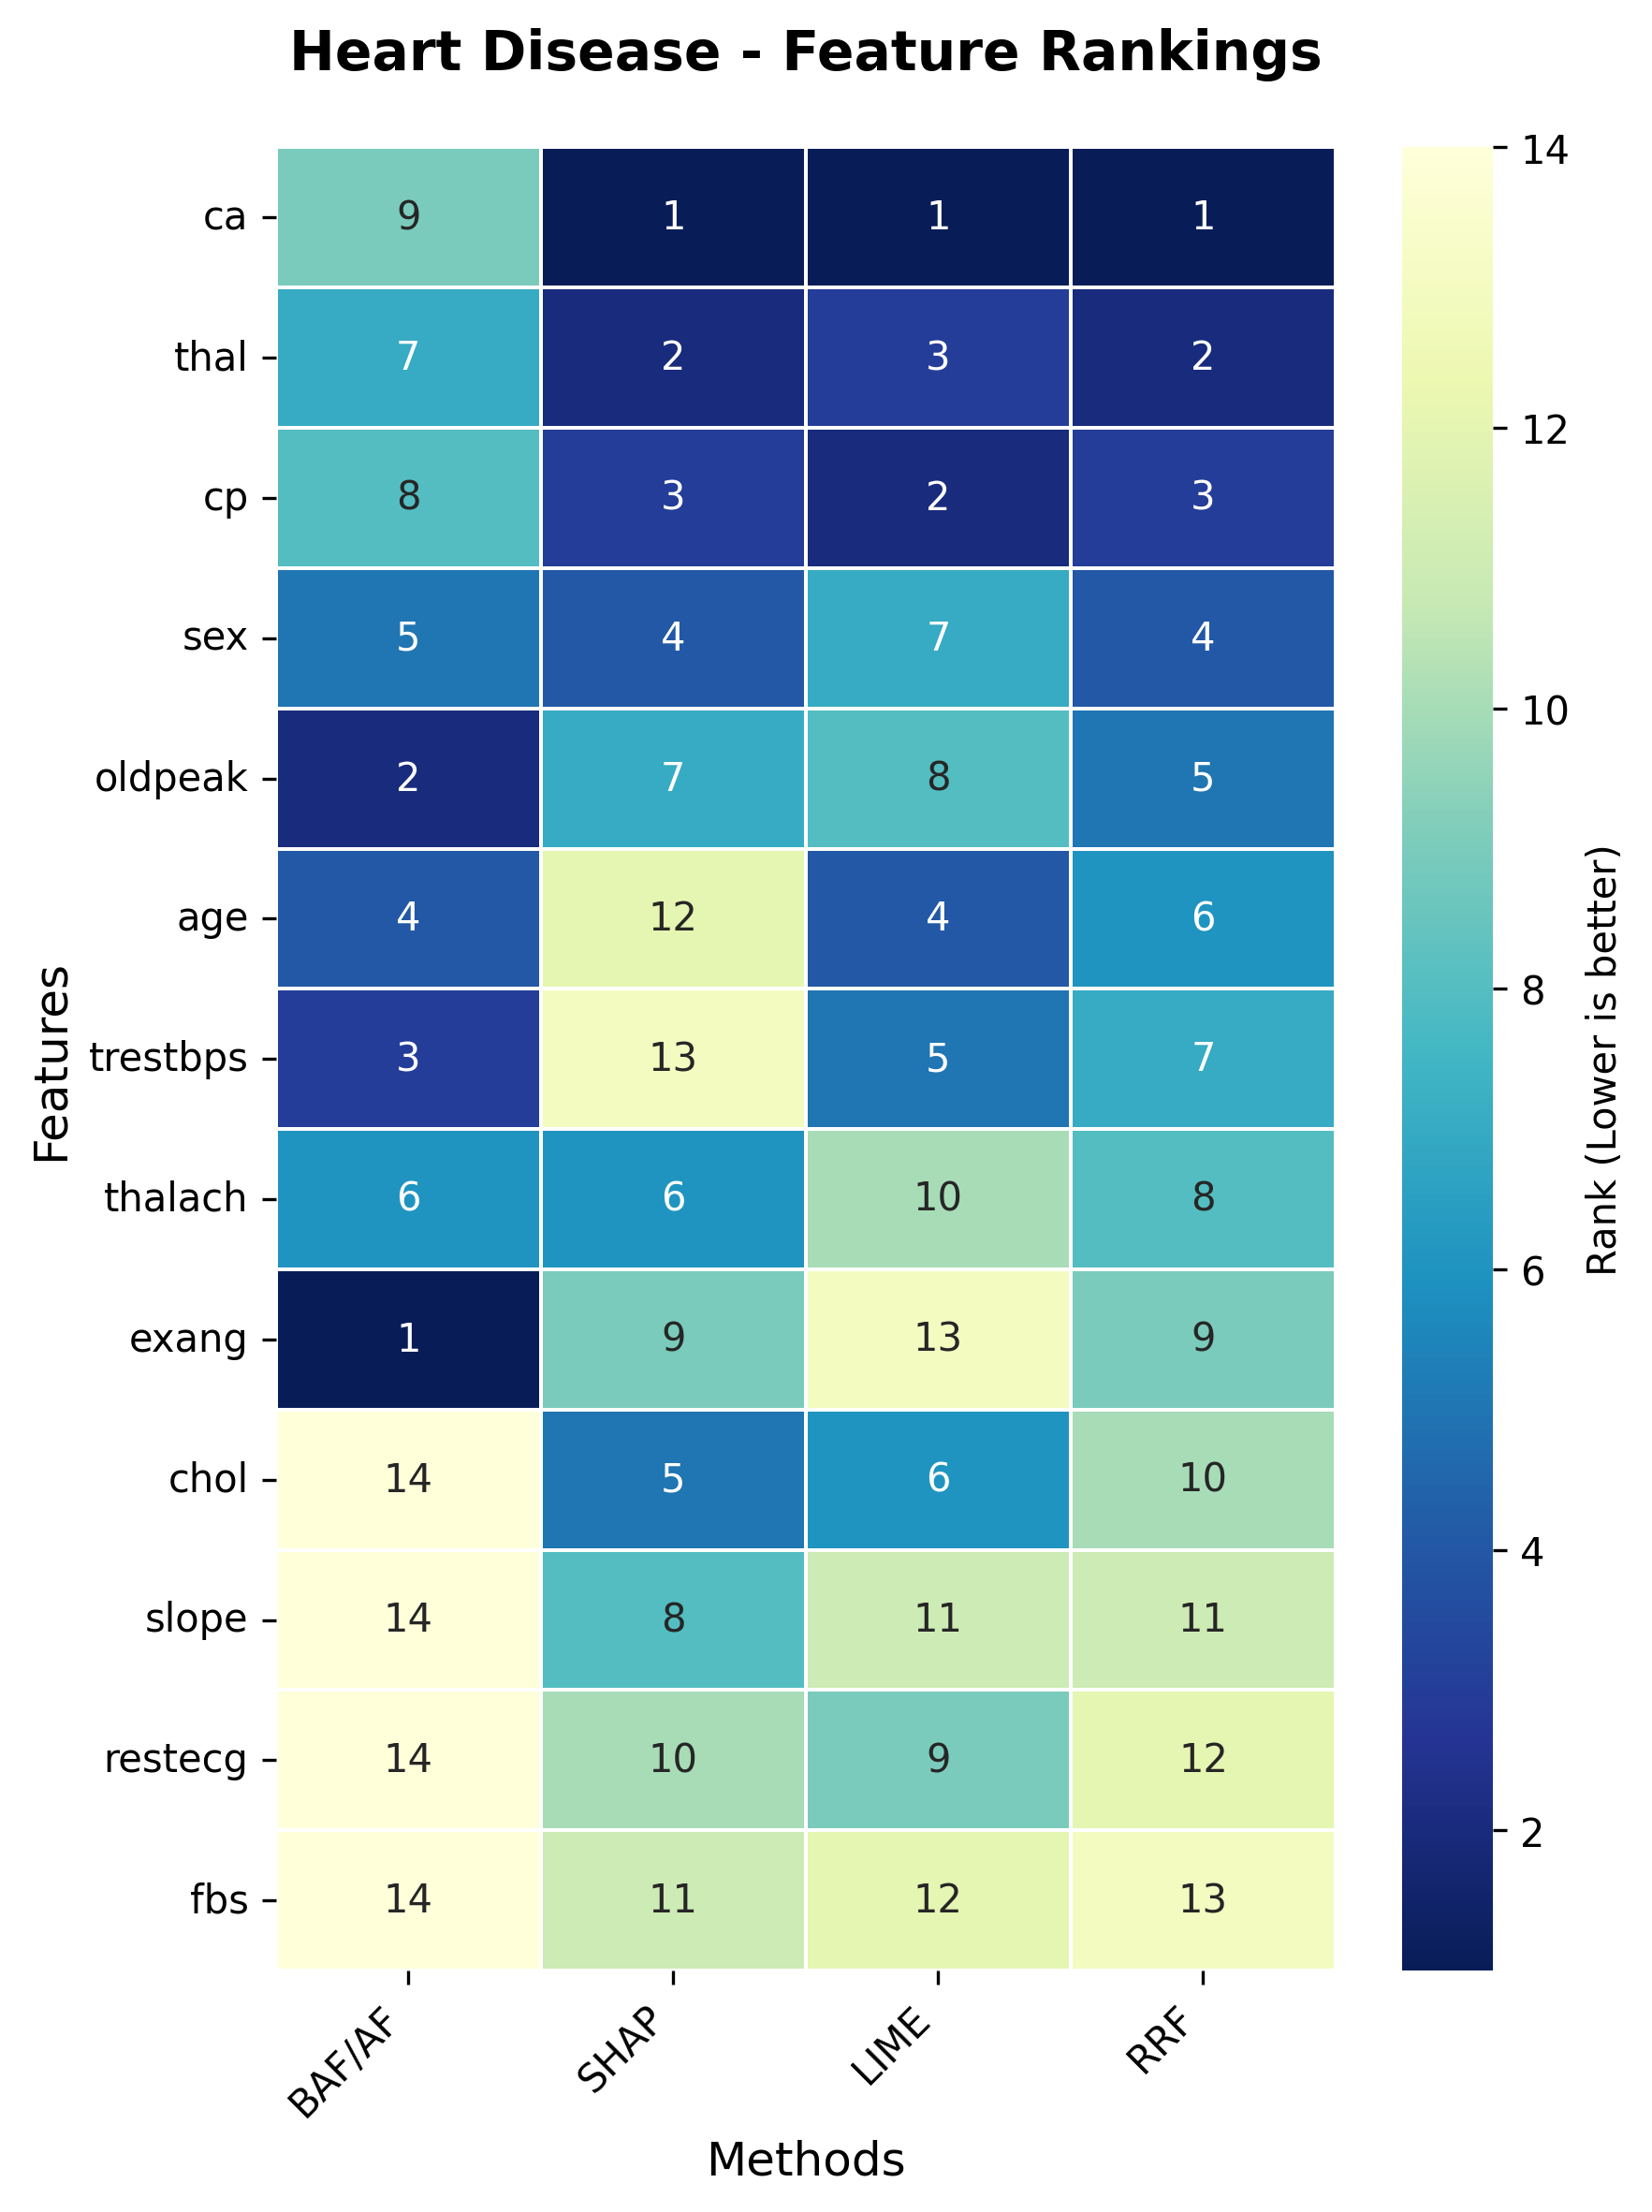
\includegraphics[width=\linewidth]{figures/rrf_rank_comparison_heart.png}
    \caption{Reciprocal Rank Fusion (RRF) comparison for the Heart Disease dataset, illustrating the stark contrast between predictive symptoms and structural causal drivers.}
    \label{fig:heart_disease_rrf}
\end{figure}

The RRF evaluation for the Pima Indians Diabetes dataset (Fig.~\ref{fig:diabetes_rrf}) demonstrated a high degree of consensus on demographic and metabolic indicators. Specifically, \texttt{Age} and \texttt{BMI} ranked consistently high across all three paradigms, achieving perfect or near-perfect consensus. However, Med-TCAX revealed structural insights that predictive methods obscured. For example, while SHAP and LIME ranked \texttt{Glucose} as the absolute strongest predictor (Rank 1), Med-TCAX ranked it lower (Rank 5) because in the causal graph, \texttt{Glucose} receives multiple argumentative attacks from higher-tier root causes. Conversely, \texttt{DiabetesPedigreeFunction}---a genetic root cause---was elevated by Med-TCAX (Rank 2) compared to predictive baselines (Rank 4). 

\begin{figure}[htbp]
    \centering
    
\includegraphics[width=\linewidth]{figures/rrf_rank_comparison.png}
    \caption{Reciprocal Rank Fusion (RRF) comparison for the Pima Indians Diabetes dataset, highlighting the alignment between causal argumentation (BAF) and predictive attributions (SHAP, LIME).}
    \label{fig:diabetes_rrf}
\end{figure}

\subsection{Discussion and Comparative Analysis}

The experimental results indicate that Med-TCAX provides stronger structural and clinical interpretability than conventional feature-attribution baselines. Rather than outperforming SHAP and LIME in predictive accuracy, the proposed framework improves the explanation process along three dimensions: causal structure, clinical plausibility, and conflict-aware reasoning.

\textbf{Transparency and Structural Awareness:} Feature-attribution methods like SHAP and LIME decompose predictions into scalar feature scores, treating inputs as independent variables. In contrast, Med-TCAX utilizes FCI to extract directed causal structures. In the Heart Disease dataset, the direct links from clinical indicators (\texttt{ca}, \texttt{cp}, \texttt{thal}) to the diagnostic target (\texttt{num}) align with SHAP importances, but Med-TCAX explicitly models the hierarchical dependencies (e.g., \texttt{Age} influencing \texttt{thalach}), transcending the limitations of mere statistical correlation.

\textbf{Clinical Plausibility:} SHAP and LIME are sensitive to correlated features and offer no guarantees against biologically impossible attributions. By enforcing tier-based constraints, Med-TCAX ensures that the generated causal directions remain semantically plausible, preventing outcomes from erroneously causing their own predictors.

\textbf{Graph-based Reasoning under Conflict:} Through the BAF and classical AF, Med-TCAX transforms raw data segments into logical "arguments," resolving conflicts via semi-stable semantics. While LIME provides static, instance-level explanations, Med-TCAX computes acceptance probabilities from generated constellations, allowing for a structured, defensible quantification of each feature's specific influence on the final clinical decision. 

\textbf{Generalizability:} The proposed framework demonstrated robust performance across two distinct pathological contexts (cardiovascular and metabolic), validating its potential for developing transparent, clinically coherent, and trustworthy Clinical Decision Support Systems (CDSS).

\section{Limitations}

Despite the promising results achieved, the proposed causal framework in this study faces several core limitations that warrant further investigation in future work.

\subsection{Dependency on Domain Expertise}
A primary drawback of this approach is its heavy reliance on domain expertise to define and organize clinical features into appropriate causal tiers. The framework requires researchers to construct a Background Knowledge graph through the manual grouping of variables. Specifically, for the UCI Heart Disease dataset, medical knowledge is essential to stratify variables, such as placing demographic factors like \texttt{Age} and \texttt{Sex} in Tier 1 (root causes), clinical indicators such as \texttt{Trestbps} and \texttt{Thalach} in Tier 2 (intermediate variables), and the diagnostic result (\texttt{Num}) in Tier 3. Similarly, establishing the causal hierarchy for the Pima Indians Diabetes dataset—including indicators such as \texttt{Pregnancies}, \texttt{Glucose}, \texttt{Insulin}, and \texttt{BMI}—necessitates direct intervention from medical professionals. This requirement significantly diminishes the framework's automation and scalability, while potentially introducing human bias if the tiered structure is inaccurately defined.

\subsection{Causal Bias from Feature Selection}
The study utilizes P-values and Random Forest (RF) feature importances to filter input attributes. However, this methodology harbors a significant theoretical flaw: P-values measure the statistical significance of linear correlations, while RF feature importances prioritize variables contributing to predictive power. Neither metric accurately reflects the underlying causal role of a variable. For instance, in the Heart Disease dataset, variables such as \texttt{fbs} and \texttt{restecg} yielded high P-values ($1.00$ and $0.083$) and low predictive importance (approximately $0.009$ and $0.021$). Removing these variables based on standard statistics risks excluding essential confounders or colliders, thereby violating the assumption of causal sufficiency and severely distorting the support or attack relations in the final causal graph.

\subsection{Computational Cost and Combinatorial Explosion}
Arising from the previous limitation, a strict trade-off exists: preserving all features to maintain the causal network immediately exposes the framework to combinatorial explosion. Applying constraint-based causal discovery algorithms (such as FCI or PC) combined with K-Fold BAF Discovery entails substantial computational overhead. As data dimensionality increases—especially following entropy-based discretization or categorical encoding—the number of arguments and attack relations in the Argumentation Framework (AF) expands rapidly.

According to the algorithmic mechanism, the \texttt{generate\_constellations} process exhibits a time complexity of $O(2^m)$, where $m$ denotes the number of significant attacks. Experimental observations indicated that the Heart Disease dataset generated 109 significant attacks (implying a search space of $2^{109}$ states), while the Diabetes dataset generated 42. This explosion necessitates approximation via random sampling and pruning (retaining only \texttt{top\_k=50} hypotheses) to prevent memory overflow. Furthermore, extracting semi-stable extensions through \texttt{\_all\_admissible\_sets()} is inherently an NP-Hard problem. This process requires traversing all combinations of the argumentation set, causing exponential growth in runtime as the feature count increases, thereby severely limiting the model's applicability to high-dimensional datasets. In practice, the framework is only tractable after reducing the feature set to a small subset, roughly 11 variables or fewer. With larger datasets, discretization and categorical encoding rapidly expand the argument space, making constellation generation and semi-stable extension computation computationally prohibitive. Therefore, feature pre-selection or dimensionality reduction is required before applying the full Med-TCAX pipeline.
\section{Conclusion and Future Work}

This paper presented Med-TCAX, a tier-constrained causal-argumentative explainability framework for clinical machine learning. Evaluated on the UCI Heart Disease dataset (303 instances, 13 features; Cleveland subset) and the Pima Indians Diabetes dataset (768 instances, 8 features), Med-TCAX demonstrated three principal contributions. First, a medical variable tiering scheme—organizing features into demographic, physiological, and outcome tiers—enforces biological precedence as forbidden-edge constraints in the FCI algorithm, significantly reducing cross-tier violations and backward temporal edges relative to unconstrained (C0) and outcome-sink-only (C1) baselines. Second, a dual-encoding strategy over entropy-discretized variables mitigates orientation instability arising from reference category selection, producing more consistent PAG structures across encoding runs. Third, a Bipolar Argumentation Framework with semi-stable extension semantics translates the constrained causal graph into structured, conflict-consistent explanations that are more clinically coherent than SHAP and LIME feature attributions.

Several directions remain open for future work. Extending the argumentation layer with counterfactual reasoning would enable clinicians to query how changing a specific variable would alter the predicted outcome, moving from descriptive to prescriptive explanation. Interventional validation using datasets with known causal ground truth—such as randomized trial data—would quantify how well tier-constrained FCI recovers true causal directions beyond observational plausibility. Replacing binary BAF polarity with probabilistic argumentation would allow uncertainty in both causal orientation and correlation magnitude to propagate into the final explanation. Finally, learning tier assignments from clinical ontologies or temporal patterns in electronic health records would reduce dependence on manually defined variable hierarchies and improve scalability to high-dimensional datasets.
% --- PHẦN TÀI LIỆU THAM KHẢO ---
% Lưu ý: Nếu bạn đang dùng lệnh \bibliography{sample} ở cuối file, 
% bạn có thể comment nó lại (thêm dấu % ở đầu) và dùng trực tiếp khối thebibliography này.
\begin{thebibliography}{99}

\bibitem{ref1} A. Rajkomar et al., ``Machine learning in medicine,'' \textit{NEJM}, vol. 380, pp. 1347–1358, 2019.
\bibitem{ref2} F. Doshi-Velez and B. Kim, ``Towards a rigorous science of interpretable machine learning,'' \textit{arXiv:1702.08608}, 2017.
\bibitem{ref3} S. M. Lundberg and S.-I. Lee, ``A unified approach to interpreting model predictions,'' \textit{NeurIPS}, 2017.
\bibitem{ref4} M. T. Ribeiro et al., ``'Why should I trust you?','' \textit{KDD}, 2016.
\bibitem{ref5} R. Prosperi et al., ``Causal inference and counterfactual prediction in machine learning for actionable healthcare,'' 
\bibitem{ref6} P. Spirtes, C. Glymour, and R. Scheines, \textit{Causation, Prediction, and Search}, MIT Press, 2000.
\bibitem{ref7} A. Beam and I. Kohane, ``Translating artificial intelligence into clinical care,'' \textit{JAMA}, vol. 316, pp. 2368–2369, 2016.
\bibitem{ref12} P. Moraffah et al., ``Causal interpretability for machine learning,'' \textit{SIGKDD Explorations}, vol. 22, 2020.
\bibitem{ref13} J. Zhang, ``On the completeness of orientation rules for causal discovery,'' \textit{Artificial Intelligence}, vol. 172, 2008.
\bibitem{ref15} A. Heskes et al., ``Causal Shapley values,'' \textit{NeurIPS}, 2020.
\bibitem{ref16} D. Heckerman et al., ``A Bayesian approach to causal discovery,'' \textit{Computation, Causation, and Discovery}, 1999.
\bibitem{ref17} C. Meek, ``Causal inference with background knowledge,'' \textit{UAI}, 1995.
\bibitem{ref18} J. Runge et al., ``Detecting causal associations in large time series datasets,'' \textit{Science Advances}, 2019.
\bibitem{ref19} R. Scheines et al., ``The TETRAD Project,'' \textit{Multivariate Behavioral Research}, vol. 33, 1998.
\bibitem{ref20} J. Rotmensch et al., ``Learning a health knowledge graph from EHR,'' \textit{Scientific Reports}, 2017.
\bibitem{ref21} P. M. Dung, ``On the acceptability of arguments,'' \textit{Artificial Intelligence}, vol. 77, pp. 321–357, 1995.
\bibitem{ref22} C. Cayrol and M.-C. Lagasquie-Schiex, ``Bipolarity in argumentation graphs,'' \textit{IJAR}, vol. 54, 2013.
\bibitem{ref23} M. W. A. Caminada, ``Semi-stable semantics,'' \textit{COMMA}, 2006.
\bibitem{ref24} K. \v{C}yras et al., ``Argumentation for explainable scheduling,'' \textit{AAAI}, 2019.
\bibitem{ref25} A. Rago et al., ``Explaining predictions by argumentation,'' \textit{AAMAS}, 2020.
\bibitem{ref26} S. Greenland et al., ``Causal diagrams for epidemiologic research,'' \textit{Epidemiology}, vol. 10, 1999.
\bibitem{ref27} D. Obermeyer and E. Emanuel, ``Predicting the future—Big data, machine learning, and clinical medicine,'' \textit{NEJM}, vol. 375, 2016.
\bibitem{ref28} J. Peters et al., \textit{Elements of Causal Inference}, MIT Press, 2017.
\bibitem{janosi1988heart}
A. Janosi, W. Steinbrunn, M. Pfisterer, and R. Detrano, ``Heart Disease,'' \textit{UCI Machine Learning Repository}, 1988. [Online]. Available: \url{https://archive.ics.uci.edu/dataset/45/heart+disease}
\bibitem{github_repo} AKANEMO22, ``causal\_argumentation\_remake\_DAP301m,'' GitHub repository. [Online]. Available: \url{https://github.com/AKANEMO22/MedTCAX-Causal-Argumentative-Explainability}
\bibitem{niddk_pima}
National Institute of Diabetes and Digestive and Kidney Diseases, ``Pima Indians Diabetes Database,'
\end{thebibliography}
\end{document}